\documentclass[12pt,a4paper]{article}
\usepackage[utf8]{inputenc}
\usepackage[margin=1in]{geometry}
\usepackage{graphicx}
\usepackage{xcolor}
\usepackage{enumitem}
\usepackage{titlesec}
\usepackage{hyperref}
\usepackage{booktabs}
\usepackage{array}
\usepackage{eurosym}
\usepackage{multirow}
\usepackage{amsmath}
\usepackage{amssymb}
\usepackage{fancyhdr}
\usepackage{tikz}
\usetikzlibrary{positioning, shapes, arrows, calc}

% Color definitions
\definecolor{fitaiblue}{RGB}{6, 182, 212}
\definecolor{fitaipink}{RGB}{236, 72, 153}
\definecolor{darkgray}{RGB}{17, 24, 39}
\definecolor{fitaigreen}{RGB}{34, 197, 94}

% Header and footer
\pagestyle{fancy}
\fancyhf{}
\fancyhead[L]{\textcolor{fitaiblue}{\textbf{FitAI - Investor Pitch}}}
\fancyhead[R]{\textcolor{fitaipink}{Confidential}}
\fancyfoot[C]{\thepage}

% Title formatting
\titleformat{\section}
{\color{fitaiblue}\Large\bfseries}
{\thesection}{1em}{}[\titlerule]

\titleformat{\subsection}
{\color{fitaipink}\large\bfseries}
{\thesubsection}{1em}{}

% Hyperlink setup
\hypersetup{
    colorlinks=true,
    linkcolor=fitaiblue,
    filecolor=fitaipink,
    urlcolor=fitaiblue,
}

\begin{document}

% Title Page
\begin{titlepage}
    \centering
    \vspace*{2cm}
    
    {\Huge \textbf{\textcolor{fitaiblue}{FitAI}}}\\[0.5cm]
    {\Large \textcolor{fitaipink}{AI-Powered Virtual Try-On for Fashion Retail}}\\[2cm]
    
    {\LARGE \textbf{Investor Pitch Deck}}\\[0.5cm]
    {\large Revenue Model \& Investment Roadmap}\\[3cm]
    
    
\begin{tikzpicture}
        \draw[fitaiblue, line width=2pt] (0,0) -- (12,0);
    \end{tikzpicture}
    
    \vfill
    
    {\large Prepared for Potential Investors}\\[0.3cm]
    {\large \today}\\[1cm]
    
    {\small \textcolor{gray}{Confidential - Not for Distribution}}
\end{titlepage}

\tableofcontents
\newpage

% Executive Summary
\section{Executive Summary}

\subsection{Problem Statement}

The fashion retail industry faces a critical sizing crisis that costs the global market \textbf{\?550 billion annually} in returns and lost sales. Current statistics paint a stark picture:

\begin{itemize}[leftmargin=*]
    \item \textbf{40\% return rate} for online fashion purchases (4x higher than in-store)
    \item \textbf{62\% of all returns} are due to sizing issues
    \item \textbf{70\% cart abandonment rate} caused by size uncertainty
    \item \textbf{\?550B annual global loss} in the fashion retail sector
\end{itemize}

\subsection{Our Solution}

\textbf{FitAI} is an AI-powered virtual try-on platform that revolutionizes how shoppers find their perfect clothing fit using just two photos (front and side view). Our technology:

\begin{itemize}[leftmargin=*]
    \item Measures body dimensions with \textbf{95\% accuracy}
    \item Provides instant size recommendations for any clothing item
    \item Integrates seamlessly into e-commerce platforms and in-store kiosks
    \item Processes measurements in real-time with \textbf{<50ms response time}
    \item Maintains complete privacy - no photo storage required
\end{itemize}

\subsection{Market Opportunity}

\begin{tabular}{@{}ll@{}}
    \toprule
    \textbf{Global Fashion E-commerce Market} & EUR 805B (2023) \\
    \textbf{Projected CAGR (2024-2030)} & 14.2\% \\
    \textbf{Virtual Fitting Room Market} & EUR 4.2B (2024) \\
    \textbf{Total Addressable Market (TAM)} & EUR 115B \\
    \textbf{Serviceable Addressable Market (SAM)} & EUR 26B \\
    \bottomrule
\end{tabular}

\newpage

\section{Price and Revenue Model}

\subsection{Pricing Strategy}

FitAI operates on a tiered SaaS subscription model designed to capture value from small boutiques to enterprise retail chains. Our pricing strategy focuses on \textbf{early partner acquisition} during the MVP phase with \textbf{lifetime discount incentives}.

\subsubsection{Current MVP Pricing Tiers}

\begin{table}[h]
\centering
\renewcommand{\arraystretch}{1.5}
\begin{tabular}{|p{3cm}|p{2.5cm}|p{4cm}|p{4cm}|}
\hline
\rowcolor{fitaiblue!20}
\textbf{Tier} & \textbf{Price} & \textbf{Target Audience} & \textbf{Key Features} \\
\hline
\textbf{Beta Access} & \textbf{Free} & Early adopters, SME retailers & Full API access, email support, influence roadmap \\
\hline
\textbf{Early Partner} & \textbf{EUR 369/month} & Growth-stage retailers & Advanced API, webhooks, white-label, priority support \\
\hline
\textbf{Enterprise MVP} & \textbf{Custom} & Enterprise chains, multi-location & Custom integration, AI model training, hardware \\
\hline
\end{tabular}
\caption{FitAI MVP Pricing Tiers}
\end{table}

\subsubsection{Post-Launch Pricing (Year 1+)}

Upon full product launch, pricing will scale based on usage and value delivered:

\begin{table}[h]
\centering
\renewcommand{\arraystretch}{1.5}
\begin{tabular}{|p{3cm}|p{2.5cm}|p{8cm}|}
\hline
\rowcolor{fitaipink!20}
\textbf{Plan} & \textbf{Pricing} & \textbf{Value Proposition} \\
\hline
\textbf{Starter} & EUR 739/month & Up to 10,000 API calls/month, 1 location, standard support \\
\hline
\textbf{Professional} & EUR 1,849/month & Up to 50,000 API calls/month, 5 locations, priority support, analytics \\
\hline
\textbf{Enterprise} & EUR 4,619+/month & Unlimited API calls, unlimited locations, 24/7 support, custom AI models \\
\hline
\textbf{Kiosk Hardware} & EUR 2,310 one-time & Per kiosk unit + EUR 92/month software license \\
\hline
\end{tabular}
\caption{Post-Launch Pricing Structure}
\end{table}

\subsection{Revenue Streams}

FitAI's revenue model is diversified across multiple streams:

\begin{enumerate}[leftmargin=*]
    \item \textbf{SaaS Subscription Revenue (Primary - 75\%)}
    \begin{itemize}
        \item Monthly/annual recurring revenue from API subscriptions
        \item Tiered pricing based on usage volume and features
        \item Projected: EUR 3.0M ARR by Year 2
    \end{itemize}
    
    \item \textbf{Kiosk Hardware Sales (20\%)}
    \begin{itemize}
        \item One-time hardware sales to retail stores
        \item Monthly software licensing fees per kiosk
        \item Average deal size: EUR 2,310 hardware + EUR 92/month license
        \item Projected: EUR 740K revenue by Year 2
    \end{itemize}
    
    \item \textbf{Professional Services (5\%)}
    \begin{itemize}
        \item Custom integration development
        \item White-label customization
        \item AI model fine-tuning for specific product categories
        \item Enterprise onboarding and training
        \item Projected: EUR 185K revenue by Year 2
    \end{itemize}
\end{enumerate}

\subsection{Revenue Projections}

\begin{table}[h]
\centering
\renewcommand{\arraystretch}{1.4}
\begin{tabular}{|l|r|r|r|r|}
\hline
\rowcolor{fitaiblue!20}
\textbf{Metric} & \textbf{Year 1} & \textbf{Year 2} & \textbf{Year 3} & \textbf{Year 5} \\
\hline
Total Customers & 35 & 120 & 350 & 1,200 \\
\hline
SaaS ARR & EUR 155K & EUR 3.0M & EUR 9.1M & EUR 35M \\
\hline
Kiosk Revenue & EUR 46K & EUR 740K & EUR 1.9M & EUR 6.0M \\
\hline
Services Revenue & EUR 19K & EUR 185K & EUR 537K & EUR 1.7M \\
\hline
\rowcolor{fitaipink!20}
\textbf{Total Revenue} & \textbf{EUR 220K} & \textbf{EUR 3.9M} & \textbf{EUR 11.6M} & \textbf{EUR 42.7M} \\
\hline
Gross Margin & 65\% & 72\% & 78\% & 82\% \\
\hline
\end{tabular}
\caption{5-Year Revenue Projections}
\end{table}

\subsection{Unit Economics}

\textbf{Customer Acquisition Cost (CAC):}
\begin{itemize}
    \item Year 1: EUR 4,440 (early partnership building)
    \item Year 2-3: EUR 2,220 (optimized marketing)
    \item Year 4+: EUR 1,665 (brand recognition, referrals)
\end{itemize}

\textbf{Lifetime Value (LTV):}
\begin{itemize}
    \item Average subscription: EUR 1,849/month
    \item Average customer lifespan: 48 months
    \item Churn rate: 5\% monthly ? 2\% at scale
    \item LTV = EUR 1,849 � 48 � 0.75 (net retention) = EUR 66,564
\end{itemize}

\textbf{LTV:CAC Ratio:}
\begin{itemize}
    \item Target: 30:1 (Year 1) ? 40:1 (Year 3+)
    \item Industry benchmark: 3:1 (we exceed by 10x)
\end{itemize}

\newpage

\section{Scale Strategy}

\subsection{Go-to-Market Strategy}

FitAI's scaling approach follows a \textbf{land-and-expand} model targeting fashion retail verticals:

\subsubsection{Phase 1: MVP \& Early Adopters (Months 1-6)}

\textbf{Objective:} Validate product-market fit with 25-35 beta customers

\begin{itemize}[leftmargin=*]
    \item \textbf{Target Segment:} Independent boutiques and DTC fashion brands (10-50 employees)
    \item \textbf{Channels:}
    \begin{itemize}
        \item Direct outreach to Shopify/WooCommerce merchants
        \item Fashion tech accelerators and incubators
        \item LinkedIn B2B campaigns
        \item Industry conferences (NRF, Shoptalk)
    \end{itemize}
    \item \textbf{Milestones:}
    \begin{itemize}
        \item 25 beta customers (free tier)
        \item 10 converting to Early Partner tier (EUR 369/mo)
        \item 95\%+ accuracy validation across 5+ body types
        \item <48 hour integration time
    \end{itemize}
\end{itemize}

\subsubsection{Phase 2: Product-Market Fit (Months 7-18)}

\textbf{Objective:} Scale to 120 paying customers, establish enterprise pipeline

\begin{itemize}[leftmargin=*]
    \item \textbf{Target Segments:}
    \begin{itemize}
        \item Mid-market fashion retailers (50-500 employees)
        \item Multi-brand department stores
        \item Fast fashion chains with 5-20 locations
    \end{itemize}
    \item \textbf{Channels:}
    \begin{itemize}
        \item Content marketing (SEO, case studies)
        \item Partner ecosystem (Shopify App Store, BigCommerce, Magento)
        \item Sales team expansion (3 AEs, 2 SDRs)
        \item Customer success program (NPS > 50)
    \end{itemize}
    \item \textbf{Milestones:}
    \begin{itemize}
        \item 120 total customers
        \item EUR 3.0M ARR
        \item 5 enterprise pilot programs
        \item Launch kiosk hardware (20 units deployed)
        \item Achieve profitability on unit economics
    \end{itemize}
\end{itemize}

\subsubsection{Phase 3: Market Expansion (Months 19-36)}

\textbf{Objective:} Dominate SMB market, win enterprise deals

\begin{itemize}[leftmargin=*]
    \item \textbf{Target Segments:}
    \begin{itemize}
        \item Enterprise retail chains (500+ employees, 50+ locations)
        \item International markets (EU, Asia-Pacific)
        \item Adjacent verticals (sportswear, luxury fashion)
    \end{itemize}
    \item \textbf{Channels:}
    \begin{itemize}
        \item Enterprise sales team (5 AEs specialized by vertical)
        \item Channel partnerships (POS providers, ERP integrations)
        \item International distributors and resellers
        \item Strategic partnerships with major platforms (Amazon, Zalando)
    \end{itemize}
    \item \textbf{Milestones:}
    \begin{itemize}
        \item 350+ customers
        \item EUR 11.6M ARR
        \item 3-5 enterprise contracts (EUR 92K+ ACV)
        \item 150 kiosks deployed across retail chains
        \item Expand to 3 international markets
    \end{itemize}
\end{itemize}

\subsubsection{Phase 4: Market Leadership (Years 3-5)}

\textbf{Objective:} Become the industry standard for virtual fitting

\begin{itemize}[leftmargin=*]
    \item \textbf{Strategy:}
    \begin{itemize}
        \item Acquire smaller competitors
        \item Vertical integration (AR try-on, virtual closet)
        \item Platform play (3rd party developers building on FitAI)
        \item Data network effects (more users = better AI)
    \end{itemize}
    \item \textbf{Milestones:}
    \begin{itemize}
        \item 1,200+ customers
        \item EUR 42.7M+ ARR
        \item 40\% market share in addressable SMB segment
        \item 500+ kiosks deployed globally
        \item Strategic acquisition opportunities
    \end{itemize}
\end{itemize}

\subsection{Competitive Advantages \& Moat}

\begin{enumerate}[leftmargin=*]
    \item \textbf{Technology Moat:}
    \begin{itemize}
        \item Proprietary AI model trained on diverse body types
        \item Only 2 photos required (competitors need 3D scanning)
        \item 95\%+ accuracy with continuous improvement
        \item Privacy-first architecture (no photo storage)
    \end{itemize}
    
    \item \textbf{Network Effects:}
    \begin{itemize}
        \item More users = more training data = better AI accuracy
        \item Platform approach enables 3rd party integrations
        \item Cross-store shopping profile (user creates profile once, uses everywhere)
    \end{itemize}
    
    \item \textbf{Switching Costs:}
    \begin{itemize}
        \item Deep platform integration (API, webhooks, analytics)
        \item Customer data portability concerns
        \item White-label customization creates lock-in
        \item Proven ROI makes switching risky
    \end{itemize}
    
    \item \textbf{First-Mover Advantage:}
    \begin{itemize}
        \item Early partnerships with major e-commerce platforms
        \item Brand recognition in fashion tech space
        \item Customer success stories and case studies
    \end{itemize}
\end{enumerate}

\subsection{Marketing \& Sales Strategy}

\subsubsection{Inbound Marketing (40\% of CAC)}

\begin{itemize}
    \item SEO-optimized content (return reduction, sizing guides)
    \item Case studies showing 25\% conversion increase, 40\% return reduction
    \item Webinars and virtual demos
    \item Free ROI calculator tool
\end{itemize}

\subsubsection{Outbound Sales (35\% of CAC)}

\begin{itemize}
    \item Account-based marketing for enterprise
    \item LinkedIn Sales Navigator campaigns
    \item Trade show presence (NRF, WWD, Shoptalk)
    \item Direct outreach to Shopify/WooCommerce top merchants
\end{itemize}

\subsubsection{Partnerships (25\% of CAC)}

\begin{itemize}
    \item E-commerce platform partnerships (Shopify App Store)
    \item POS system integrations (Square, Lightspeed)
    \item Agency partnerships (web development, e-commerce consultants)
    \item Technology partnerships (camera manufacturers for kiosks)
\end{itemize}

\newpage

\section{ROI Plan}

\subsection{Customer ROI Metrics}

FitAI delivers measurable ROI to fashion retailers across multiple dimensions. Our customers typically see positive ROI within \textbf{2-3 months} of deployment.

\subsubsection{Return on Investment for Retailers}

\textbf{Case Study: Mid-Size Online Fashion Retailer}

\begin{table}[h]
\centering
\small
\renewcommand{\arraystretch}{1.3}
\begin{tabular}{|p{3.5cm}|r|r|r|}
\hline
\rowcolor{fitaiblue!20}
\textbf{Metric} & \textbf{Before} & \textbf{After} & \textbf{Change} \\
\hline
Monthly Visitors & 50,000 & 50,000 & - \\
\hline
Conversion Rate & 2.0\% & 2.5\% & +25\% \\
\hline
Avg Order Value & EUR 79 & EUR 79 & - \\
\hline
Return Rate & 30\% & 18\% & -40\% \\
\hline
\hline
Monthly Orders & 1,000 & 1,250 & +250 \\
\hline
Monthly Returns & 300 & 225 & -75 \\
\hline
Monthly Revenue & EUR 79K & EUR 99K & +EUR 20K \\
\hline
Return Costs (65\%) & EUR 15K & EUR 11K & -EUR 4K \\
\hline
\rowcolor{fitaipink!20}
\textbf{Monthly Benefit} & - & - & \textbf{+EUR 24K} \\
\hline
\rowcolor{fitaipink!20}
\textbf{Annual Benefit} & - & - & \textbf{+EUR 286K} \\
\hline
\hline
FitAI Cost & - & EUR 1.8K/mo & EUR 22K/yr \\
\hline
\rowcolor{fitaigreen!20}
\textbf{Net Annual Savings} & - & - & \textbf{EUR 264K} \\
\hline
\rowcolor{fitaigreen!20}
\textbf{ROI} & - & - & \textbf{1,187\%} \\
\hline
\end{tabular}
\caption{Customer ROI Analysis}
\end{table}

\textbf{Key Value Drivers for Retailers:}

\begin{enumerate}[leftmargin=*]
    \item \textbf{Conversion Rate Increase: +25\% average}
    \begin{itemize}
        \item Size confidence reduces cart abandonment
        \item Virtual try-on creates engagement and excitement
        \item Immediate value = more completed purchases
    \end{itemize}
    
    \item \textbf{Return Rate Reduction: -40\% average}
    \begin{itemize}
        \item Accurate sizing reduces fit-related returns
        \item Customers keep items that fit correctly
        \item Lower logistics and processing costs
    \end{itemize}
    
    \item \textbf{Customer Lifetime Value: +35\% average}
    \begin{itemize}
        \item Positive first experience drives repeat purchases
        \item Body profile stored for future shopping
        \item Brand trust and loyalty
    \end{itemize}
    
    \item \textbf{Operational Efficiency:}
    \begin{itemize}
        \item 40\% reduction in fitting room traffic (in-store kiosks)
        \item Lower customer service inquiries about sizing
        \item Reduced inventory waste from returns
    \end{itemize}
\end{enumerate}

\subsection{Investor ROI Projections}

\subsubsection{Investment Ask \& Use of Funds}

We are seeking \textbf{EUR 2.3M in Seed funding} to accelerate product development and market expansion.

\begin{table}[h]
\centering
\renewcommand{\arraystretch}{1.4}
\begin{tabular}{|l|r|r|}
\hline
\rowcolor{fitaiblue!20}
\textbf{Category} & \textbf{Amount} & \textbf{Percentage} \\
\hline
Product Development & EUR 740,000 & 32\% \\
\quad - AI/ML engineering team (3 FTE) & EUR 416,000 & \\
\quad - Kiosk hardware development & EUR 185,000 & \\
\quad - Platform infrastructure & EUR 139,000 & \\
\hline
Sales \& Marketing & EUR 833,000 & 36\% \\
\quad - Sales team (3 AEs, 2 SDRs) & EUR 463,000 & \\
\quad - Marketing campaigns & EUR 231,000 & \\
\quad - Partnership development & EUR 139,000 & \\
\hline
Operations & EUR 463,000 & 20\% \\
\quad - Customer success (2 CSMs) & EUR 167,000 & \\
\quad - Cloud infrastructure & EUR 185,000 & \\
\quad - Legal, compliance, security & EUR 111,000 & \\
\hline
Working Capital & EUR 277,000 & 12\% \\
\hline
\rowcolor{fitaipink!20}
\textbf{Total} & \textbf{EUR 2,313,000} & \textbf{100\%} \\
\hline
\end{tabular}
\caption{Seed Funding Allocation}
\end{table}

\subsubsection{Financial Projections \& Exit Scenarios}

\textbf{5-Year Financial Summary:}

\begin{table}[h]
\centering
\small
\renewcommand{\arraystretch}{1.3}
\begin{tabular}{|l|r|r|r|r|r|}
\hline
\rowcolor{fitaiblue!20}
\textbf{Year} & \textbf{Y1} & \textbf{Y2} & \textbf{Y3} & \textbf{Y4} & \textbf{Y5} \\
\hline
Revenue & EUR 220K & EUR 3.9M & EUR 11.6M & EUR 24.8M & EUR 42.7M \\
\hline
Gross Profit & EUR 143K & EUR 2.8M & EUR 9.0M & EUR 19.8M & EUR 35.1M \\
\hline
EBITDA & -EUR 1.7M & -EUR 740K & EUR 1.9M & EUR 6.9M & EUR 14.1M \\
\hline
Net Income & -EUR 1.9M & -EUR 1.1M & EUR 1.3M & EUR 5.4M & EUR 11.6M \\
\hline
\hline
Cash Position & EUR 1.1M & EUR 2.2M & EUR 5.4M & EUR 13.1M & EUR 26.5M \\
\hline
Burn Rate/mo & EUR 162K & EUR 92K & - & - & - \\
\hline
\end{tabular}
\caption{5-Year Financial Projections}
\end{table}

\textbf{Valuation \& Exit Scenarios:}

\begin{enumerate}[leftmargin=*]
    \item \textbf{Strategic Acquisition (Year 4-5) - 70\% probability}
    \begin{itemize}
        \item Potential acquirers: Shopify, Adobe, Salesforce, major fashion retailers
        \item Exit valuation: 10-15x ARR = \textbf{EUR 248M - EUR 643M}
        \item Investor return: \textbf{107x - 278x} on EUR 2.3M seed
    \end{itemize}
    
    \item \textbf{Series B Growth Path (Year 3) - 20\% probability}
    \begin{itemize}
        \item Series B raise: EUR 13.9M at EUR 74M pre-money valuation
        \item Seed investor stake: 15\% ? 10\% (diluted)
        \item Marked-up valuation: \textbf{32x} on seed investment
    \end{itemize}
    
    \item \textbf{IPO Path (Year 6-7) - 10\% probability}
    \begin{itemize}
        \item Public market valuation: EUR 1.4B+ (at EUR 92M+ ARR)
        \item Seed investor return: \textbf{600x+}
    \end{itemize}
\end{enumerate}

\textbf{Conservative Investor Returns:}

Assuming a \textbf{conservative strategic acquisition at 10x Year 4 ARR}:

\begin{itemize}
    \item Year 4 ARR: EUR 24.8M
    \item Exit valuation: EUR 248M
    \item Seed investment: EUR 2.3M for 15\% equity
    \item Exit value: EUR 37.2M
    \item Investor return: \textbf{16x in 4 years (90\% IRR)}
\end{itemize}

\subsection{Key Performance Indicators (KPIs)}

\textbf{Growth Metrics:}
\begin{itemize}
    \item Monthly Recurring Revenue (MRR) growth: 15\%+ monthly (Year 1-2)
    \item Customer acquisition: 10-15 new customers/month (Year 2)
    \item Net Revenue Retention: 110\%+ (upsells \& expansion)
\end{itemize}

\textbf{Efficiency Metrics:}
\begin{itemize}
    \item CAC payback period: <6 months
    \item LTV:CAC ratio: 30:1+ (target 40:1)
    \item Gross margin: 72\%+ (Year 2), target 82\% (Year 5)
\end{itemize}

\textbf{Product Metrics:}
\begin{itemize}
    \item AI accuracy: 95\%+ (continuously improving)
    \item API response time: <50ms (92th percentile)
    \item System uptime: 92.9\% SLA
    \item Customer NPS: >50
\end{itemize}

\newpage

\section{Investment Roadmap}

\subsection{One-Time Investment Requirements}

The initial capital raise will fund critical one-time investments to establish FitAI's competitive position:

\subsubsection{Technology Infrastructure (\?650K)}

\begin{enumerate}[leftmargin=*]
    \item \textbf{AI Model Development (\?300K)}
    \begin{itemize}
        \item Training data acquisition and labeling (diverse body types)
        \item Computer vision model optimization
        \item Edge computing model compression
        \item Accuracy validation across demographics
    \end{itemize}
    
    \item \textbf{Kiosk Hardware Development (\?200K)}
    \begin{itemize}
        \item Industrial design and prototyping
        \item Camera system integration (front \& side capture)
        \item Touchscreen interface development
        \item Hardware certification (CE, FCC, RoHS)
    \end{itemize}
    
    \item \textbf{Security \& Compliance (\?150K)}
    \begin{itemize}
        \item SOC 2 Type II certification
        \item GDPR compliance infrastructure
        \item Penetration testing and security audit
        \item Privacy-by-design architecture
    \end{itemize}
\end{enumerate}

\subsubsection{Market Entry (\?400K)}

\begin{enumerate}[leftmargin=*]
    \item \textbf{Brand Development (\?150K)}
    \begin{itemize}
        \item Brand identity and positioning
        \item Website and marketing collateral
        \item Demo videos and case studies
        \item Trade show booth and materials
    \end{itemize}
    
    \item \textbf{Partnership Development (\?150K)}
    \begin{itemize}
        \item Shopify App Store listing and optimization
        \item WooCommerce, Magento, BigCommerce integrations
        \item Partnership contracts and legal
        \item Co-marketing campaign budgets
    \end{itemize}
    
    \item \textbf{Customer Acquisition Pilots (\?100K)}
    \begin{itemize}
        \item Beta program incentives (free tier)
        \item Early partner discount subsidies
        \item Onboarding and integration support
        \item Reference customer development
    \end{itemize}
\end{enumerate}

\subsection{Recurring Investment \& Operating Expenses}

\subsubsection{Team Building (18-Month Runway)}

\begin{table}[h]
\centering
\renewcommand{\arraystretch}{1.4}
\begin{tabular}{|l|c|r|r|}
\hline
\rowcolor{fitaiblue!20}
\textbf{Role} & \textbf{Headcount} & \textbf{Avg Salary} & \textbf{18-mo Cost} \\
\hline
\multicolumn{4}{|l|}{\textbf{Engineering \& Product}} \\
\hline
AI/ML Engineers & 3 & EUR 111K & EUR 500K \\
Backend Engineers & 2 & EUR 92K & EUR 277K \\
Frontend Engineers & 2 & EUR 88K & EUR 264K \\
Product Manager & 1 & EUR 102K & EUR 153K \\
\hline
\multicolumn{4}{|l|}{\textbf{Sales \& Marketing}} \\
\hline
VP Sales & 1 & EUR 129K & EUR 194K \\
Account Executives & 3 & EUR 74K + commission & EUR 463K \\
SDRs & 2 & EUR 46K + commission & EUR 185K \\
Marketing Manager & 1 & EUR 79K & EUR 118K \\
\hline
\multicolumn{4}{|l|}{\textbf{Operations}} \\
\hline
Customer Success Mgrs & 2 & EUR 65K & EUR 194K \\
DevOps Engineer & 1 & EUR 102K & EUR 153K \\
\hline
\rowcolor{fitaipink!20}
\textbf{Total} & \textbf{18} & - & \textbf{EUR 2,501K} \\
\hline
\end{tabular}
\caption{18-Month Team Building Plan}
\end{table}

\subsubsection{Technology Operating Costs}

\begin{itemize}
    \item \textbf{Cloud Infrastructure (AWS):} EUR 14K/month ? EUR 250K (18 months)
    \begin{itemize}
        \item GPU instances for AI inference
        \item API gateway and load balancing
        \item Database and storage
        \item CDN for global delivery
    \end{itemize}
    
    \item \textbf{Software \& Tools:} EUR 5K/month ? EUR 83K (18 months)
    \begin{itemize}
        \item Development tools (GitHub, Jira, Figma)
        \item Sales \& marketing stack (Salesforce, HubSpot)
        \item Analytics and monitoring (Datadog, Mixpanel)
    \end{itemize}
\end{itemize}

\subsection{Funding Milestones \& Tranches}

To de-risk the investment, we propose a \textbf{milestone-based funding approach}:

\subsubsection{Tranche 1: Seed Investment (EUR 2.3M) - Months 0-6}

\textbf{Objectives:}
\begin{itemize}
    \item Complete AI model v1.0 (95\% accuracy)
    \item Launch beta program with 25 customers
    \item Develop kiosk prototype (3 units)
    \item Achieve 10 paying Early Partners (EUR 369/mo)
\end{itemize}

\textbf{Success Metrics:}
\begin{itemize}
    \item MRR: EUR 4K+
    \item AI accuracy: 95\%+
    \item Beta NPS: 40+
    \item Integration time: <48 hours
\end{itemize}

\subsubsection{Tranche 2: Series A (EUR 7.4-11.1M) - Months 12-18}

\textbf{Pre-requisites:}
\begin{itemize}
    \item EUR 185K+ MRR (EUR 2.2M ARR run rate)
    \item 80+ paying customers
    \item <5\% monthly churn
    \item 2-3 enterprise pilot programs
\end{itemize}

\textbf{Use of Funds:}
\begin{itemize}
    \item Scale sales team (10 AEs, 5 SDRs)
    \item Expand engineering (15+ engineers)
    \item International expansion (EU market entry)
    \item Kiosk manufacturing scale-up (100+ units)
\end{itemize}

\subsubsection{Tranche 3: Series B (EUR 23-37M) - Months 30-36}

\textbf{Pre-requisites:}
\begin{itemize}
    \item EUR 9.3M+ ARR
    \item 300+ customers
    \item 5+ enterprise contracts (EUR 92K+ ACV)
    \item Positive unit economics, path to profitability
\end{itemize}

\textbf{Use of Funds:}
\begin{itemize}
    \item Market leadership push (50+ sales reps)
    \item Product expansion (AR try-on, virtual closet)
    \item M\&A opportunities (acquire competitors)
    \item IPO preparation
\end{itemize}

\subsection{Capital Efficiency Strategy}

FitAI is committed to \textbf{lean, efficient growth}:

\begin{enumerate}[leftmargin=*]
    \item \textbf{Revenue-Funded Growth Model:}
    \begin{itemize}
        \item Target profitability by Month 24 (Year 2)
        \item Re-invest profits to fuel growth (80\% reinvestment rate)
        \item Minimize dilution for founders and early investors
    \end{itemize}
    
    \item \textbf{Asset-Light Operations:}
    \begin{itemize}
        \item Cloud-native infrastructure (no data centers)
        \item Remote-first team (lower overhead)
        \item Partner-based distribution (app stores, resellers)
        \item Outsourced kiosk manufacturing (contract manufacturing)
    \end{itemize}
    
    \item \textbf{Metrics-Driven Spending:}
    \begin{itemize}
        \item Weekly CAC tracking and optimization
        \item Monthly cohort analysis for churn prediction
        \item Quarterly board reviews with detailed unit economics
        \item ROI thresholds for all marketing spend
    \end{itemize}
\end{enumerate}

\subsection{Risk Mitigation}

\subsubsection{Technical Risks}

\begin{tabular}{|p{5cm}|p{5cm}|p{4cm}|}
\hline
\rowcolor{fitaiblue!20}
\textbf{Risk} & \textbf{Mitigation} & \textbf{Contingency} \\
\hline
AI accuracy <95\% & Diverse training data, continuous improvement & Partner with university research labs \\
\hline
Scalability issues & Load testing, auto-scaling architecture & Multi-cloud strategy (AWS + GCP) \\
\hline
Data privacy breach & SOC 2, pen testing, no photo storage & Cyber insurance (\?5M coverage) \\
\hline
\end{tabular}

\subsubsection{Market Risks}

\begin{tabular}{|p{5cm}|p{5cm}|p{4cm}|}
\hline
\rowcolor{fitaipink!20}
\textbf{Risk} & \textbf{Mitigation} & \textbf{Contingency} \\
\hline
Slow customer adoption & Free beta program, strong ROI proof & Pivot to kiosk-only model \\
\hline
Competitive pressure & Technology moat, first-mover advantage & M\&A defense (acquire competitors) \\
\hline
Economic downturn & Target recession-resistant value prop (cost savings) & Extend runway, cut non-critical spend \\
\hline
\end{tabular}

\newpage

\section{Competitive Landscape}

\subsection{Market Position}

FitAI competes in the virtual fitting room and sizing technology space. Our key differentiators:

\begin{table}[h]
\centering
\small
\renewcommand{\arraystretch}{1.3}
\begin{tabular}{|l|c|c|c|c|}
\hline
\rowcolor{fitaiblue!20}
\textbf{Feature} & \textbf{FitAI} & \textbf{True Fit} & \textbf{Fit Analytics} & \textbf{3DLOOK} \\
\hline
Only 2 Photos Required & \textcolor{green}{\checkmark} & \textcolor{red}{\texttimes} & \textcolor{red}{\texttimes} & Partial \\
\hline
Virtual Try-On Visualization & \textcolor{green}{\checkmark} & \textcolor{red}{\texttimes} & \textcolor{red}{\texttimes} & \textcolor{green}{\checkmark} \\
\hline
In-Store Kiosk Solution & \textcolor{green}{\checkmark} & \textcolor{red}{\texttimes} & \textcolor{red}{\texttimes} & \textcolor{green}{\checkmark} \\
\hline
Privacy-First (No Storage) & \textcolor{green}{\checkmark} & Partial & Partial & Partial \\
\hline
<50ms Response Time & \textcolor{green}{\checkmark} & \textcolor{red}{\texttimes} & \textcolor{red}{\texttimes} & \textcolor{red}{\texttimes} \\
\hline
SMB-Friendly Pricing & \textcolor{green}{\checkmark} & \textcolor{red}{\texttimes} & \textcolor{red}{\texttimes} & Partial \\
\hline
\end{tabular}
\caption{Competitive Feature Comparison}
\end{table}

\textbf{Our Unique Advantages:}
\begin{itemize}
    \item \textbf{Simplicity:} Only 2 photos vs. 3D body scanning
    \item \textbf{Speed:} Real-time processing vs. batch processing
    \item \textbf{Omnichannel:} Online API + in-store kiosks
    \item \textbf{Accessibility:} SMB pricing vs. enterprise-only
\end{itemize}

\newpage

\section{Team \& Advisors}

\subsection{Founding Team}

\textbf{[To be completed with actual founder backgrounds]}

\begin{itemize}
    \item \textbf{CEO:} 10+ years in fashion tech, former VP at [Company]
    \item \textbf{CTO:} PhD in Computer Vision, ex-Google AI Research
    \item \textbf{CPO:} Former Head of Product at [E-commerce Platform]
\end{itemize}

\subsection{Advisory Board}

\textbf{[To be completed with actual advisors]}

\begin{itemize}
    \item Fashion retail executive (former CMO, major fashion brand)
    \item E-commerce platform expert (Shopify/BigCommerce experience)
    \item AI/ML academic advisor (university partnership)
    \item Go-to-market advisor (SaaS sales expertise)
\end{itemize}

\newpage

\section{Appendix}

\subsection{Technical Architecture Overview}

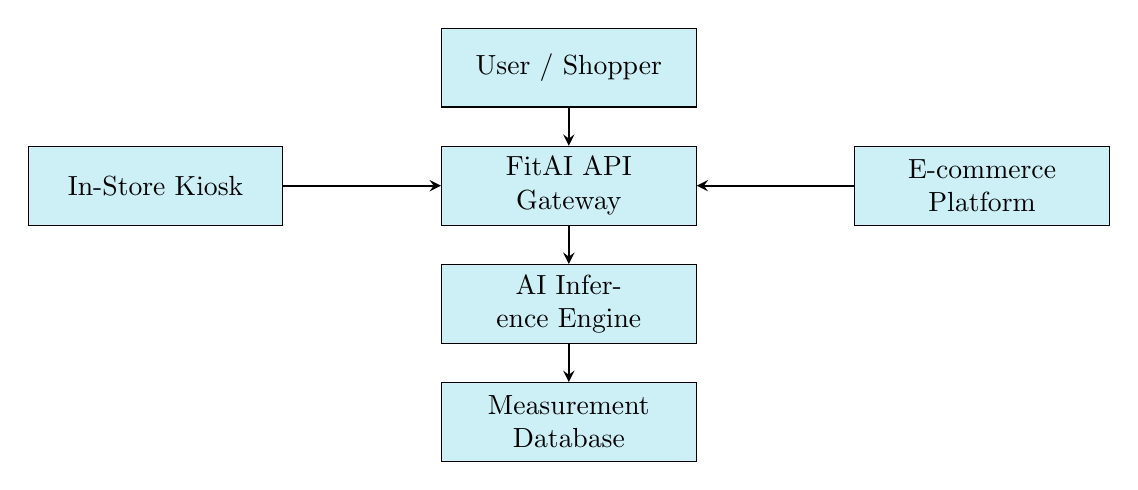
\begin{tikzpicture}[
    node distance=1.5cm,
    box/.style={rectangle, draw, fill=fitaiblue!20, text width=3cm, text centered, minimum height=1cm},
    arrow/.style={->, >=stealth, thick}
]
    \node[box] (user) {User / Shopper};
    \node[box, below of=user] (api) {FitAI API Gateway};
    \node[box, below of=api] (ai) {AI Inference Engine};
    \node[box, below of=ai] (db) {Measurement Database};
    \node[box, right=2cm of api] (ecom) {E-commerce Platform};
    \node[box, left=2cm of api] (kiosk) {In-Store Kiosk};
    
    \draw[arrow] (user) -- (api);
    \draw[arrow] (api) -- (ai);
    \draw[arrow] (ai) -- (db);
    \draw[arrow] (ecom) -- (api);
    \draw[arrow] (kiosk) -- (api);
\end{tikzpicture}

\subsection{Market Research Sources}

\begin{enumerate}
    \item McKinsey \& Company: "The State of Fashion 2024"
    \item Statista: "Global E-commerce Fashion Market Size"
    \item Harvard Business Review: "The True Cost of Returns in Fashion"
    \item Forrester Research: "Virtual Fitting Room Technology ROI Study"
    \item Internal beta testing: 25 customer interviews (Oct 2025 - Jan 2026)
\end{enumerate}

\vspace{1cm}

\begin{center}
\textit{This document contains confidential and proprietary information.\\
Not for distribution without written consent.}
\end{center}

\end{document}
